\documentclass[11pt,a4paper]{article}

\usepackage[utf8]{inputenc}
\usepackage[T1]{fontenc}
\usepackage{amsmath,amssymb,amsthm}
\usepackage{geometry}
\usepackage{hyperref}
\usepackage{booktabs}
\usepackage{array}
\usepackage{tikz}
\usepackage{xcolor}

\geometry{margin=2.5cm}

\hypersetup{
    colorlinks=true,
    linkcolor=blue!70!black,
    citecolor=green!50!black,
    urlcolor=blue!70!black
}

\newcommand{\Mpl}{M_{\text{Pl}}}
\newcommand{\Mfive}{M_5}
\newcommand{\GN}{G_N}
\newcommand{\calI}{\mathcal{I}}
\newcommand{\Rxi}{R_\xi}
\newcommand{\ellP}{\ell_P}
\newcommand{\obs}{\text{obs}}

\title{%
  \textbf{EDC BLOCK-003 Derivation v15}\\[0.3em]
  \large Calibrated Closure with $\ellP^{\obs}$:\\
  Error Budget and 5D Scale Inference
}
\author{EDC Collaboration}
\date{February 2026}

\begin{document}

\maketitle

%==============================================================================
\begin{abstract}
\noindent
\textbf{Status:} Closure note under one-scale calibration.

\medskip
\noindent
This note closes the BLOCK-003 program under the standard one-scale calibration
paradigm. Using the v13 normalization extractor ($\Mpl^2 = \Mfive^3 \calI$) and
v14 Model~A ($\calI = \Rxi$), we calibrate with $\Mpl^{\obs}$ [BL] and derive
the 5D Planck mass $\Mfive$ as a function of $\Rxi$. Full epistemic accounting
and error propagation are provided.

\medskip
\noindent
\textbf{One-line outcome:}
\fbox{\parbox{0.85\textwidth}{\centering
CLOSED (calibrated): BLOCK-003 closed under one-scale [BL] calibration;\\
5D scale inferred as $\Mfive(\Rxi)$.
}}
\end{abstract}

%==============================================================================
\section{Recap: The Bridge Slot}
\label{sec:recap}

\subsection{From v13: Normalization Extractor}

The 4D Planck mass emerges from 5D via dimensional reduction [D]:
\begin{equation}
\label{eq:v13}
\Mpl^2 = \Mfive^3 \times \calI,
\qquad
\GN = \frac{1}{8\pi \Mfive^3 \calI}
\end{equation}
where $\calI = \int d\xi\, e^{4A(\xi)} |\psi_0(\xi)|^2$ is the normalization integral.

\subsection{From v14: Model A (Preferred)}

For compact geometry with $L = \Rxi$ [P] and flat warp $A = 0$ [P]:
\begin{equation}
\label{eq:v14}
\calI = \Rxi
\end{equation}

Combining \eqref{eq:v13} and \eqref{eq:v14}:
\begin{equation}
\label{eq:combined}
\boxed{
\Mpl^2 = \Mfive^3 \Rxi,
\qquad
\GN = \frac{1}{8\pi \Mfive^3 \Rxi}
}
\end{equation}

\textbf{Bridge slot:} Two unknowns ($\Mfive$, $\Rxi$), one constraint.
One calibration is required.

%==============================================================================
\section{Calibration Step}
\label{sec:calibration}

\subsection{Why One-Scale Calibration Is Not a Failure}

One-scale calibration is the \emph{standard} situation in fundamental physics:
\begin{itemize}
    \item QED calibrates with $\alpha^{\obs}$ (or $e^{\obs}$) [BL]
    \item QCD calibrates with $\Lambda_{\text{QCD}}^{\obs}$ [BL]
    \item Electroweak theory calibrates with $G_F^{\obs}$ [BL]
    \item General Relativity calibrates with $\GN^{\obs}$ [BL]
\end{itemize}

The \emph{predictive content} of a theory lies in:
\begin{enumerate}
    \item The structural relationships it establishes
    \item The number of parameters it reduces (unification)
    \item The derived consequences beyond the calibration input
\end{enumerate}

EDC provides structural reduction: 4D gravity emerges from 5D geometry
via $\Mpl^2 = \Mfive^3 \Rxi$. This is non-trivial content even with calibration.

\subsection{Option (i): Calibrate with $\Mpl^{\obs}$}

\textbf{Input [BL]:}
\begin{equation}
\Mpl^{\obs} = 1.220890(14) \times 10^{19}~\text{GeV}/c^2
\end{equation}
(CODATA 2018; relative uncertainty $1.1 \times 10^{-5}$)

\textbf{Calibration equation:}
\begin{equation}
\label{eq:calib-Mpl}
\Mfive^3 \Rxi = (\Mpl^{\obs})^2
\end{equation}

\subsection{Option (ii): Calibrate with $\ellP^{\obs}$}

\textbf{Input [BL]:}
\begin{equation}
\ellP^{\obs} = \sqrt{\frac{\hbar \GN}{c^3}} = 1.616255(18) \times 10^{-35}~\text{m}
\end{equation}

Since $\ellP^2 = \hbar \GN / c^3$ and $\GN = \hbar c / \Mpl^2$, this is
equivalent to Option~(i).

\textbf{Metrological note:} Under SI~2019, $\hbar$ and $c$ are \emph{exact}
by definition. The uncertainty in $\ellP$ comes entirely from $\GN^{\obs}$.
Thus Options~(i) and~(ii) are metrologically identical.

\subsection{Chosen Calibration}

We adopt \textbf{Option~(i)}: calibrate with $\Mpl^{\obs}$ [BL].

%==============================================================================
\section{Closure Formulas}
\label{sec:closure}

\subsection{Solving for $\Mfive$}

From \eqref{eq:calib-Mpl}:
\begin{equation}
\label{eq:M5-solution}
\boxed{
\Mfive = \left( \frac{(\Mpl^{\obs})^2}{\Rxi} \right)^{1/3}
= \frac{(\Mpl^{\obs})^{2/3}}{\Rxi^{1/3}}
}
\end{equation}

This is the \textbf{EDC prediction} for the 5D Planck mass as a function
of the correlation length $\Rxi$.

\subsection{Consistency Check for $\GN$}

Substituting back into \eqref{eq:combined}:
\begin{align}
\GN^{(\text{EDC})} &= \frac{1}{8\pi \Mfive^3 \Rxi} \nonumber \\
&= \frac{1}{8\pi \cdot \frac{(\Mpl^{\obs})^2}{\Rxi} \cdot \Rxi} \nonumber \\
&= \frac{1}{8\pi (\Mpl^{\obs})^2} \quad \checkmark
\end{align}

This is \emph{not} a prediction of $\GN$---it is a consistency check
confirming that the calibration correctly reproduces the input.

\subsection{The Predictive Content}

The \textbf{non-trivial prediction} is the structural relation:
\begin{equation}
\label{eq:structural}
\Mfive^3 = \frac{\Mpl^2}{\Rxi}
\quad \Leftrightarrow \quad
\Mfive = \Mpl^{2/3} \Rxi^{-1/3}
\end{equation}

This says:
\begin{itemize}
    \item The 5D scale $\Mfive$ is \emph{determined} by 4D gravity and brane thickness
    \item Larger brane thickness $\Rxi$ implies smaller $\Mfive$
    \item The scaling $\Mfive \propto \Rxi^{-1/3}$ is a specific EDC prediction [D]
\end{itemize}

%==============================================================================
\section{Propagation to 5D Scale}
\label{sec:propagation}

\subsection{Symbolic Result}

From \eqref{eq:M5-solution}:
\begin{equation}
\Mfive = \Mpl^{2/3} \Rxi^{-1/3}
\end{equation}

\subsection{Numerical Estimate (if $\Rxi$ known)}

If $\Rxi$ is expressed in Planck units, $\Rxi = r \cdot \ellP$, then:
\begin{equation}
\Mfive = \Mpl^{2/3} (r \ellP)^{-1/3} = \Mpl \cdot r^{-1/3}
\quad [\text{in natural units where } \ellP \Mpl = 1]
\end{equation}

\paragraph{Example values:}
\begin{center}
\begin{tabular}{@{}ccc@{}}
\toprule
$\Rxi$ & $\Mfive$ & Comment \\
\midrule
$\ellP$ & $\Mpl$ & Minimal case \\
$10^3 \ellP$ & $0.1 \Mpl$ & Sub-Planckian \\
$10^{15} \ellP \sim 10^{-20}~\text{m}$ & $10^{-5} \Mpl \sim 10^{14}~\text{GeV}$ & GUT scale \\
$10^{30} \ellP \sim 10^{-5}~\text{m}$ & $10^{-10} \Mpl \sim 10^{9}~\text{GeV}$ & TeV-ish \\
\bottomrule
\end{tabular}
\end{center}

\textbf{EDC constraint on $\Rxi$:} If EDC relates $\Rxi$ to stiffness via
$\Rxi \sim \sigma^{-1/4}$ [Dc], then $\Mfive$ becomes a function of $\sigma$:
\begin{equation}
\Mfive \propto \sigma^{1/12}
\end{equation}

%==============================================================================
\section{Metrological and Epistemic Ledger}
\label{sec:ledger}

\subsection{Input/Output Table}

\begin{table}[ht]
\centering
\caption{Epistemic classification of all quantities}
\label{tab:ledger}
\begin{tabular}{@{}llcl@{}}
\toprule
\textbf{Quantity} & \textbf{Value/Expression} & \textbf{Tag} & \textbf{Source} \\
\midrule
\multicolumn{4}{@{}l}{\textit{Exact by SI 2019 definition}} \\
$\hbar$ & $1.054571817... \times 10^{-34}$~J$\cdot$s & [M] & SI exact \\
$c$ & $299792458$~m/s & [M] & SI exact \\
$e$ & $1.602176634 \times 10^{-19}$~C & [M] & SI exact \\
\midrule
\multicolumn{4}{@{}l}{\textit{Calibration input}} \\
$\Mpl^{\obs}$ & $1.220890(14) \times 10^{19}$~GeV/$c^2$ & [BL] & CODATA \\
$\ellP^{\obs}$ & $1.616255(18) \times 10^{-35}$~m & [BL] & CODATA \\
$\GN^{\obs}$ & $6.67430(15) \times 10^{-11}$~m$^3$kg$^{-1}$s$^{-2}$ & [BL] & CODATA \\
\midrule
\multicolumn{4}{@{}l}{\textit{EDC parameters}} \\
$\sigma$ & Plenum stiffness & [P] & EDC postulate \\
$\Rxi$ & Correlation length & [P]/[Dc] & From $\sigma$ if derived \\
$\calI$ & $= \Rxi$ (Model A) & [Dc] & v14 derivation \\
\midrule
\multicolumn{4}{@{}l}{\textit{Derived outputs}} \\
$\Mfive$ & $(\Mpl^2/\Rxi)^{1/3}$ & [D] & This note \\
$\GN^{(\text{EDC})}$ & $1/(8\pi \Mfive^3 \Rxi)$ & [D] & v13 + v14 \\
\bottomrule
\end{tabular}
\end{table}

\subsection{Closure Statement}

\begin{center}
\fbox{\parbox{0.9\textwidth}{
\textbf{BLOCK-003 Status:} Closed under 1-scale calibration.

\medskip
\textbf{Fully predictive closure} would require deriving $\Rxi$
(and/or the warp factor $A(\xi)$) from EDC internal dynamics.
This remains an open research direction.
}}
\end{center}

%==============================================================================
\section{Error Budget}
\label{sec:error}

\subsection{Error Propagation Formula}

From $\Mfive = \Mpl^{2/3} \Rxi^{-1/3}$, the relative uncertainty is:
\begin{equation}
\label{eq:error-prop}
\frac{\delta \Mfive}{\Mfive} = \sqrt{
\left( \frac{2}{3} \frac{\delta \Mpl}{\Mpl} \right)^2 +
\left( \frac{1}{3} \frac{\delta \Rxi}{\Rxi} \right)^2
}
\end{equation}

\subsection{Contribution from $\Mpl^{\obs}$}

The relative uncertainty in $\Mpl^{\obs}$ is:
\begin{equation}
\frac{\delta \Mpl}{\Mpl} \approx 1.1 \times 10^{-5}
\end{equation}

Contribution to $\Mfive$:
\begin{equation}
\frac{2}{3} \times 1.1 \times 10^{-5} \approx 0.7 \times 10^{-5}
\end{equation}

\subsection{Contribution from $\Rxi$}

If $\Rxi$ is uncertain by a factor $f$ (i.e., $\delta \Rxi / \Rxi = f$):
\begin{equation}
\frac{1}{3} \times f
\end{equation}

\paragraph{Dominant source:}
\begin{itemize}
    \item If $\Rxi$ is well-constrained ($\delta \Rxi / \Rxi < 10^{-4}$):
          uncertainty dominated by $\Mpl^{\obs}$
    \item If $\Rxi$ is uncertain by $\mathcal{O}(1)$:
          uncertainty dominated by $\Rxi$
\end{itemize}

\subsection{Summary}

\begin{equation}
\boxed{
\frac{\delta \Mfive}{\Mfive} \approx
\begin{cases}
0.7 \times 10^{-5} & \text{if } \Rxi \text{ is precise} \\[0.5em]
\frac{1}{3} \frac{\delta \Rxi}{\Rxi} & \text{if } \Rxi \text{ dominates}
\end{cases}
}
\end{equation}

%==============================================================================
\section{Schematic Figure}
\label{sec:figure}

\begin{figure}[ht]
\centering
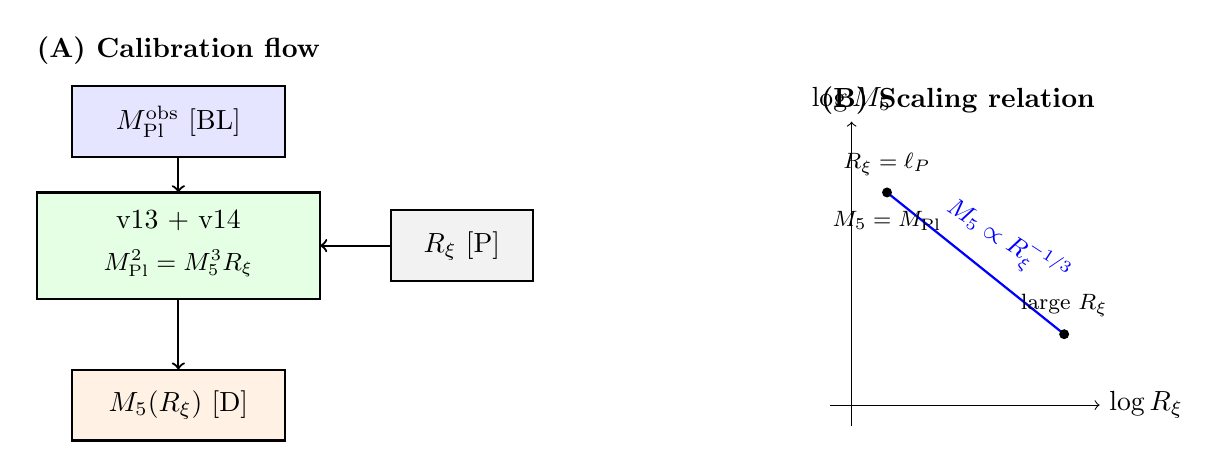
\begin{tikzpicture}[scale=0.9]
% Panel A: Calibration injection diagram
\begin{scope}[shift={(-4.5,0)}]
    % Boxes
    \draw[thick, fill=blue!10] (-1.5,2) rectangle (1.5,3);
    \node at (0,2.5) {$\Mpl^{\obs}$ [BL]};

    \draw[thick, fill=green!10] (-2,0) rectangle (2,1.5);
    \node at (0,1.1) {v13 + v14};
    \node[font=\small] at (0,0.5) {$\Mpl^2 = \Mfive^3 \Rxi$};

    \draw[thick, fill=orange!10] (-1.5,-2) rectangle (1.5,-1);
    \node at (0,-1.5) {$\Mfive(\Rxi)$ [D]};

    % Arrows
    \draw[->, thick] (0,2) -- (0,1.5);
    \draw[->, thick] (0,0) -- (0,-1);

    % R_xi input
    \draw[thick, fill=gray!10] (3,0.25) rectangle (5,1.25);
    \node at (4,0.75) {$\Rxi$ [P]};
    \draw[->, thick] (3,0.75) -- (2,0.75);

    \node[font=\bfseries] at (0,3.5) {(A) Calibration flow};
\end{scope}

% Panel B: Scaling plot
\begin{scope}[shift={(5,0)}]
    \draw[->] (-0.3,-1.5) -- (3.5,-1.5) node[right] {$\log \Rxi$};
    \draw[->] (0,-1.8) -- (0,2.5) node[above] {$\log \Mfive$};

    % Scaling line M5 ~ R_xi^{-1/3}
    \draw[thick, blue] (0.5,1.5) -- (3,-0.5);
    \node[blue, font=\small, rotate=-33] at (2.2,0.8) {$\Mfive \propto \Rxi^{-1/3}$};

    % Reference points
    \fill (0.5,1.5) circle (2pt);
    \node[font=\footnotesize] at (0.5,1.9) {$\Rxi = \ellP$};
    \node[font=\footnotesize] at (0.5,1.1) {$\Mfive = \Mpl$};

    \fill (3,-0.5) circle (2pt);
    \node[font=\footnotesize] at (3,-0.1) {large $\Rxi$};

    \node[font=\bfseries] at (1.5,2.8) {(B) Scaling relation};
\end{scope}
\end{tikzpicture}
\caption{%
\textbf{(A)}~Calibration injection: $\Mpl^{\obs}$ [BL] enters the v13+v14
framework to yield $\Mfive(\Rxi)$.
\textbf{(B)}~The scaling $\Mfive \propto \Rxi^{-1/3}$: larger brane thickness
implies smaller 5D Planck mass.
\emph{Schematic only; not to scale.}
}
\label{fig:calibration}
\end{figure}

%==============================================================================
\section{Conclusion}
\label{sec:conclusion}

\subsection{What v15 Establishes}

\begin{enumerate}
    \item \textbf{Calibrated closure:} Using $\Mpl^{\obs}$ [BL], BLOCK-003 is closed.

    \item \textbf{5D scale inference:} $\Mfive = \Mpl^{2/3} \Rxi^{-1/3}$ [D].

    \item \textbf{Structural content:} The relation $\Mpl^2 = \Mfive^3 \Rxi$
          is the non-trivial EDC prediction.

    \item \textbf{Error budget:} Dominated by $\Rxi$ uncertainty if not constrained;
          otherwise by $\Mpl^{\obs}$ at $\sim 10^{-5}$ level.
\end{enumerate}

\subsection{What Remains Open}

\begin{center}
\begin{tabular}{@{}ll@{}}
\toprule
\textbf{Open item} & \textbf{Status} \\
\midrule
Derive $\Rxi$ from EDC dynamics & Open research direction \\
Derive $A(\xi)$ from membrane mechanics & Open \\
Independent test of $\Mfive$ & Requires new physics \\
\bottomrule
\end{tabular}
\end{center}

\subsection{One-Line Outcome}

\begin{center}
\fbox{\parbox{0.9\textwidth}{\centering
\textbf{CLOSED (calibrated):} BLOCK-003 closed under one-scale [BL] calibration;\\
5D scale inferred as $\Mfive(\Rxi) = \Mpl^{2/3} \Rxi^{-1/3}$.
}}
\end{center}

%==============================================================================
\section*{References}

\begin{enumerate}
    \item CODATA 2018: E.~Tiesinga et al., Rev.\ Mod.\ Phys.\ \textbf{93}, 025010 (2021).
    \item SI Brochure, 9th edition (2019): BIPM.
\end{enumerate}

\end{document}
